\documentclass[9pt]{beamer}
\beamertemplatenavigationsymbolsempty
\usetheme{Berlin}

\usepackage{etex, tikz, array, graphics, xspace, relsize, multirow}
\usepackage{ulem}

\input binhex

% For code inclusion
\usepackage{listings}
\lstset{ breaklines=true}
\lstset{escapeinside={<@}{@>}}
\usepackage{algorithm2e}
\usepackage{algorithmic}

% Commands
\newcommand\A{\mathcal{A}}
\newcommand\cc{\mathcal{C}}
\newcommand\codim{\mathrm{codim}}
\newcommand\CP{\mathbb{CP}}
\newcommand\C{\mathbb{C}}
\newcommand\D{\mathrm{D}}
\newcommand\hto{\hookrightarrow}
\newcommand\I{^{-1}}
\newcommand\oo{\mathcal{O}}
\renewcommand\phi{\varphi}
\newcommand\Pj{\mathbb{P}}
\newcommand\pow{\mathcal{P}}
\newcommand\RP{\mathbb{RP}}
\newcommand\rstr[2]{{\left.#1\right|_{#2}}}
\newcommand\R{\mathbb{R}}
\newcommand\V{\mathcal{V}}
\newcommand\F{\mathcal{F}}
\newcommand\G{\mathcal{G}}
\newcommand\Graph{\G(\F_{\mathcal{L}, b}, G)}
\newcommand\set[1]{\{#1\}}
\newcommand\toi{\xrightarrow{\sim}} % category
\newcommand\Z{\mathbb{Z}}


% For drawing
%% Tikz drawing
\usepackage{tikz}
\usetikzlibrary{arrows}
\usetikzlibrary{arrows.meta}
\usepackage{pgfplots}
\usepackage{tikz-3dplot}
\usepackage{tcolorbox}
\usetikzlibrary{matrix,fit,positioning,shapes.geometric,patterns,backgrounds}
\usetikzlibrary{decorations.pathreplacing}
\usetikzlibrary{decorations.markings}
\usetikzlibrary{arrows,calc}
\tikzstyle{bigbox} = [draw=blue!50, thick, rounded corners, rectangle]
\tikzset{
>=stealth'
}
\tikzset{->-/.style={decoration={
  markings,
  mark=at position #1 with {\arrow{>}}},postaction={decorate}}}

%% Software names
\newcommand\topcom{\texttt{TOPCOM}\xspace}
\newcommand\mptopcom{\texttt{MPTOPCOM}\xspace}
\newcommand\mptopcomone{\texttt{MPTOPCOM-1}\xspace}
\newcommand\mts{\texttt{mts}\xspace}
\newcommand\mplrs{\texttt{mplrs}\xspace}
\newcommand\soplex{\texttt{soplex}\xspace}
\newcommand\openmpi{\texttt{OpenMPI}\xspace}
\newcommand\mpi{\texttt{MPI}\xspace}
\newcommand\gfan{\texttt{Gfan}\xspace}
\newcommand\cddlib{\texttt{cddlib}\xspace}
\newcommand\polydb{\texttt{PolyDB}\xspace}
\newcommand\OSCAR{\texttt{OSCAR}\xspace}
\newcommand\Julia{\texttt{Julia}\xspace}

\usepackage{xcolor}
\definecolor{green}{rgb}{0.1,0.59,0.1}
\definecolor{yellow}{rgb}{0.8,0.67,0}
\definecolor{red}{rgb}{0.89,0.1,0.1}
\definecolor{blue}{rgb}{0.1,0.1,0.89}

\usenavigationsymbolstemplate{}

\usepackage{booktabs}
% For software citations
\newcommand{\polymake}{\texttt{po\-ly\-ma\-ke}\xspace}
\newcommand{\polymakejl}{\texttt{Po\-ly\-ma\-ke.jl}\xspace}
\newcommand{\singular}{\texttt{Sin\-gu\-lar}\xspace}
\newcommand\CPP{C\nolinebreak\hspace{-.05em}\raisebox{.4ex}{\relsize{-3}{\textbf{+}}}\nolinebreak\hspace{-.10em}\raisebox{.4ex}{\relsize{-3}{\textbf{+}}}\xspace}

\usepackage{amsmath}
% Newcommands specifically for this article
\newcommand{\eval}{v}               % evaluation function giving switch table
\newcommand{\graph}{\Gamma}         % reverse search graph
\newcommand{\group}{G}              % group acting on point config
\newcommand{\groupElem}{g}          % element of group
\newcommand{\jbound}{\psi}          % bound on the number of elements of set J
\newcommand{\switchTableSize}{\mu}  % index of last non-trivial row in switch table

\newcommand{\pc}{\mathcal P\mathcal C}
\newcommand{\ZZ}{\mathbb Z}
\renewcommand{\AA}{\mathcal A}
\newcommand{\QQ}{\mathbb Q}
\newcommand{\OO}{\mathcal O}
\newcommand{\CC}{\mathbb C}
\newcommand{\PP}{\mathbb P}
\newcommand{\RR}{\mathbb R}
\newcommand{\scalp}[1]{\langle #1 \rangle}
\newcommand{\wt}{\omega}
\newcommand{\cT}{\mathcal T}
\renewcommand{\O}{\mathcal O}
\newcommand{\adm}{\mathcal A(\D, M)}
\newcommand{\blue}[1]{{\usebeamercolor[fg]{palette primary}#1}}

\DeclareMathOperator{\CaDiv}{CaDiv}
\DeclareMathOperator{\conv}{conv}
\DeclareMathOperator{\below}{defect}
\DeclareMathOperator{\vertex}{vertex}
\DeclareMathOperator{\Cox}{Cox}
\DeclareMathOperator{\cl}{cl}
\DeclareMathOperator{\cone}{cone}
\DeclareMathOperator{\Ext}{Ext}
\DeclareMathOperator{\Tor}{Tor}
\DeclareMathOperator{\lcm}{lcm}
\DeclareMathOperator{\Quot}{Quot}
\DeclareMathOperator{\Spec}{Spec}
\DeclareMathOperator{\Sets}{Sets}
\DeclareMathOperator{\relint}{relint}
\DeclareMathOperator{\rk}{rk}
\DeclareMathOperator{\smallestFace}{smallestFace}
\DeclareMathOperator{\Pic}{Pic}
\DeclareMathOperator{\Hom}{Hom}
\DeclareMathOperator{\vol}{vol}
\DeclareMathOperator{\TV}{TV}
\DeclareMathOperator{\tail}{tail}
\DeclareMathOperator{\rep}{rep}
\DeclareMathOperator{\vspan}{span}
\DeclareMathOperator{\canonical}{can}
\DeclareMathOperator{\gkz}{gkz}

\newcommand{\pmsmall}{\includegraphics[scale=0.03]{pmlogo.png}}
\newcommand{\pmlogo}{\includegraphics[scale=0.09]{pmlogo.png}}
\newcommand{\pmbluesmall}{\includegraphics[scale=0.03]{pmbluelogo.png}}
\newcommand{\Disjoint}{\mathop{\coprod}}
\newcommand{\Discriminant}{\mathcal{D}}

\theoremstyle{definition}
\newtheorem{remark}{Remark}

\newtheorem{lem}{Lemma}
\newtheorem{defn}{Definition}

\author{Antony Della Vecchia}
\title{Building Software Infrastructure for Research Mathematics}
%\newtheorem*{example}{Example}
\institute[]{
Technische Universit\"at Berlin
}
\date{
2024-06-20
}
\logo{
  \includegraphics[width=2cm]{images/mardi-logo.png}
}


\newcommand{\surj}{\twoheadrightarrow}
\newcommand{\oursetting}[1]{\textcolor{blue}{#1}}
\usepackage{listings}
\begin{document}
\maketitle
%%%%%%%%%%%%%%%%%%%%%%%%%%%%%%%%%%%%%%%%%%%%%%%%%%%%%%%%%%%%%%%%%%%%%%%%%%%%%%%
%%%%%%%%%%%%%%%%%%%%%%%%%%%%%%%%%%%%%%%%%%%%%%%%%%%%%%%%%%%%%%%%%%%%%%%%%%%%%%%
%%%%%%%%%%%%%%%%%%%%%%%%%%%%%%%%%%%%%%%%%%%%%%%%%%%%%%%%%%%%%%%%%%%%%%%%%%%%%%%


\begin{frame}[fragile]{Overview}
  \begin{itemize}
  \item MaRDI and the FAIR Principles
  \item Serialization and Datasets
  \item \Julia and \OSCAR
  \end{itemize}
\end{frame}


%%%%%%%%%%%%%%%%%%%%%%%%%%%%%%%%%%%%%%%%%%%%%%%%%%%%%%%%%%%%%%%%%%%%%%%%%%%%%%%
%%%%%%%%%%%%%%%%%%%%%%%%%%%%%%%%%%%%%%%%%%%%%%%%%%%%%%%%%%%%%%%%%%%%%%%%%%%%%%%
%%%%%%%%%%%%%%%%%%%%%%%%%%%%%%%%%%%%%%%%%%%%%%%%%%%%%%%%%%%%%%%%%%%%%%%%%%%%%%%


\begin{frame}[fragile]{The FAIR Principles}
  \begin{tcolorbox}
    \begin{itemize}
    \item Findable
    \item Accessible
    \item Interoperable
    \item Reusable
    \end{itemize}
    \end{tcolorbox}
    
\end{frame}

%%%%%%%%%%%%%%%%%%%%%%%%%%%%%%%%%%%%%%%%%%%%%%%%%%%%%%%%%%%%%%%%%%%%%%%%%%%%%%%
%%%%%%%%%%%%%%%%%%%%%%%%%%%%%%%%%%%%%%%%%%%%%%%%%%%%%%%%%%%%%%%%%%%%%%%%%%%%%%%
%%%%%%%%%%%%%%%%%%%%%%%%%%%%%%%%%%%%%%%%%%%%%%%%%%%%%%%%%%%%%%%%%%%%%%%%%%%%%%%


\begin{frame}[fragile]{MaRDI}

  \begin{itemize}
  \item Develop a mathematical research data infrastructure.
  \item Set standards for confirmable workflows and certified mathematical research data.
  \item Provide services to both the mathematical and wider scientific community.
  \end{itemize}
  \begin{center}
    \includegraphics[width=0.5\textwidth, height=0.5\textheight]{images/graph}
  \end{center}

\end{frame}

%%%%%%%%%%%%%%%%%%%%%%%%%%%%%%%%%%%%%%%%%%%%%%%%%%%%%%%%%%%%%%%%%%%%%%%%%%%%%%%
%%%%%%%%%%%%%%%%%%%%%%%%%%%%%%%%%%%%%%%%%%%%%%%%%%%%%%%%%%%%%%%%%%%%%%%%%%%%%%%
%%%%%%%%%%%%%%%%%%%%%%%%%%%%%%%%%%%%%%%%%%%%%%%%%%%%%%%%%%%%%%%%%%%%%%%%%%%%%%%


\begin{frame}[fragile]{Why Files?}
  \begin{itemize}
  \item People often have a preferred software system. \pause
  \item Computations can be expensive. \pause
  \item Verification of results is at most as computationally expensive.\pause
  \item Software changes often. 
  \end{itemize}
\end{frame}

%%%%%%%%%%%%%%%%%%%%%%%%%%%%%%%%%%%%%%%%%%%%%%%%%%%%%%%%%%%%%%%%%%%%%%%%%%%%%%%
%%%%%%%%%%%%%%%%%%%%%%%%%%%%%%%%%%%%%%%%%%%%%%%%%%%%%%%%%%%%%%%%%%%%%%%%%%%%%%%
%%%%%%%%%%%%%%%%%%%%%%%%%%%%%%%%%%%%%%%%%%%%%%%%%%%%%%%%%%%%%%%%%%%%%%%%%%%%%%%

\begin{frame}[fragile]{Storing Mathematical Data}
  \begin{itemize}
    \item It's common to have multiple perspectives on an object in mathematics. \pause
    \item While storing mathematical data a choice of perspective must me made. \pause
    \end{itemize}

  Say we want to store:
  \begin{align*}
    p(x, y, z) = xy - z^2
  \end{align*} \pause

  \begin{itemize}
  \item Some technicalities with the coefficients.
  \item Is x considered as a coefficient of y?
  \end{itemize}
\end{frame}

%%%%%%%%%%%%%%%%%%%%%%%%%%%%%%%%%%%%%%%%%%%%%%%%%%%%%%%%%%%%%%%%%%%%%%%%%%%%%%%
%%%%%%%%%%%%%%%%%%%%%%%%%%%%%%%%%%%%%%%%%%%%%%%%%%%%%%%%%%%%%%%%%%%%%%%%%%%%%%%
%%%%%%%%%%%%%%%%%%%%%%%%%%%%%%%%%%%%%%%%%%%%%%%%%%%%%%%%%%%%%%%%%%%%%%%%%%%%%%%

\begin{frame}[fragile]{ Storing LPs}

  \begin{tabular}{cl}  
    \begin{tabular}{c}
      \includegraphics[height=4cm, width=2.5cm]{images/lp_file}
      \includegraphics[height=4cm, width=2.5cm]{images/mps_file}
    \end{tabular}
    & \begin{tabular}{l}
        \parbox{0.5\linewidth}{%  change the parbox width as appropiate

          \begin{itemize}
          \item LPs heavily used in industry.
          \item Industry natural define standards.
          \item The LP file format, the MPS file format. 
          \end{itemize}
        }
      \end{tabular}  \\
  \end{tabular}
\end{frame}

%%%%%%%%%%%%%%%%%%%%%%%%%%%%%%%%%%%%%%%%%%%%%%%%%%%%%%%%%%%%%%%%%%%%%%%%%%%%%%%
%%%%%%%%%%%%%%%%%%%%%%%%%%%%%%%%%%%%%%%%%%%%%%%%%%%%%%%%%%%%%%%%%%%%%%%%%%%%%%%
%%%%%%%%%%%%%%%%%%%%%%%%%%%%%%%%%%%%%%%%%%%%%%%%%%%%%%%%%%%%%%%%%%%%%%%%%%%%%%%

\begin{frame}[fragile]{The Polymake File Format}
  
  \begin{tabular}{cl}  
    \begin{tabular}{c}
      \includegraphics[height=6cm, width=4cm]{images/xml_file}
    \end{tabular}
    & \begin{tabular}{l}
        \parbox{0.5\linewidth}{%  change the parbox width as appropiate
        \begin{itemize}
        \item First version (XML) published in 2016.
        \end{itemize}
        }
      \end{tabular}  \\
  \end{tabular}
\end{frame}

\begin{frame}[fragile]{The Polymake File Format}
  \begin{tabular}{cl}  
    \begin{tabular}{c}
      \includegraphics[height=6cm, width=4cm]{images/json_file}
    \end{tabular}
    & \begin{tabular}{l}
        \parbox{0.5\linewidth}{%  change the parbox width as appropiate
        \begin{itemize}
        \item First version (XML) published in 2016. 
        \item Currently using JSON.\pause
        \item Builds on already existing infrastructure. \pause
        \item Extensible, tree structure. \pause
        \item Has a Schema. \pause
        \item Older formats will be upgraded on load. \pause
        \item Can be loaded into OSCAR and SAGE. 
        \end{itemize}
        }
      \end{tabular}  \\
  \end{tabular}
\end{frame}


%%%%%%%%%%%%%%%%%%%%%%%%%%%%%%%%%%%%%%%%%%%%%%%%%%%%%%%%%%%%%%%%%%%%%%%%%%%%%%%
%%%%%%%%%%%%%%%%%%%%%%%%%%%%%%%%%%%%%%%%%%%%%%%%%%%%%%%%%%%%%%%%%%%%%%%%%%%%%%%
%%%%%%%%%%%%%%%%%%%%%%%%%%%%%%%%%%%%%%%%%%%%%%%%%%%%%%%%%%%%%%%%%%%%%%%%%%%%%%%

\begin{frame}[fragile]{Tree Structure}
  \begin{figure}
    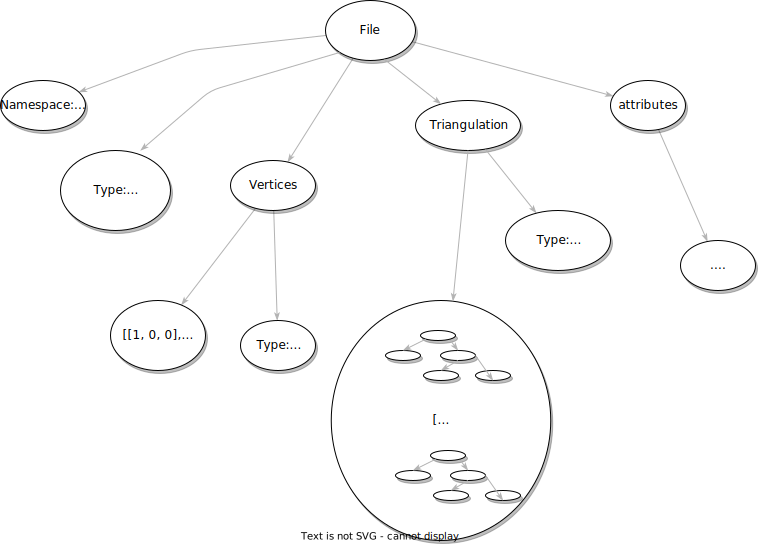
\includegraphics[width=.9\textwidth, height=0.86\textheight]{images/tree-diagram}
  \end{figure}
\end{frame}

%%%%%%%%%%%%%%%%%%%%%%%%%%%%%%%%%%%%%%%%%%%%%%%%%%%%%%%%%%%%%%%%%%%%%%%%%%%%%%%
%%%%%%%%%%%%%%%%%%%%%%%%%%%%%%%%%%%%%%%%%%%%%%%%%%%%%%%%%%%%%%%%%%%%%%%%%%%%%%%
%%%%%%%%%%%%%%%%%%%%%%%%%%%%%%%%%%%%%%%%%%%%%%%%%%%%%%%%%%%%%%%%%%%%%%%%%%%%%%%


\begin{frame}[fragile]{Schemata}
  \begin{itemize}
  \item A schema defines a general structure for data so that it can be interpreted by software. \pause
  \item Schema languages. \pause
  \item Is possible to define recursive structure. \pause
  \item Can be generated from software. \pause
  \item Schemata allow data to be validated without being read into software. \pause
  \item Adds structure to document based databases.
  \end{itemize}
\end{frame}

%%%%%%%%%%%%%%%%%%%%%%%%%%%%%%%%%%%%%%%%%%%%%%%%%%%%%%%%%%%%%%%%%%%%%%%%%%%%%%%
%%%%%%%%%%%%%%%%%%%%%%%%%%%%%%%%%%%%%%%%%%%%%%%%%%%%%%%%%%%%%%%%%%%%%%%%%%%%%%%
%%%%%%%%%%%%%%%%%%%%%%%%%%%%%%%%%%%%%%%%%%%%%%%%%%%%%%%%%%%%%%%%%%%%%%%%%%%%%%%

\begin{frame}[fragile]{On Going Work}
    \begin{tabular}{cl}  
    \begin{tabular}{c}
      \includegraphics[height=6cm, width=4cm]{images/oscar_file}
    \end{tabular}
    & \begin{tabular}{l}
        \parbox{0.5\linewidth}{%  change the parbox width as appropiate
        \begin{itemize}
        \item Prototyping in OSCAR. \pause
        \item Aim to be software independant. \pause
        \item Functionality for storing most types in OSCAR. \pause
        \item Julia package for small databases. 
        \end{itemize}
        }
      \end{tabular}  \\
  \end{tabular}
\end{frame}

%%%%%%%%%%%%%%%%%%%%%%%%%%%%%%%%%%%%%%%%%%%%%%%%%%%%%%%%%%%%%%%%%%%%%%%%%%%%%%%
%%%%%%%%%%%%%%%%%%%%%%%%%%%%%%%%%%%%%%%%%%%%%%%%%%%%%%%%%%%%%%%%%%%%%%%%%%%%%%%
%%%%%%%%%%%%%%%%%%%%%%%%%%%%%%%%%%%%%%%%%%%%%%%%%%%%%%%%%%%%%%%%%%%%%%%%%%%%%%%

\begin{frame}[fragile]{}
  \frametitle{References}
  \begin{center}
    Thank You!
  \end{center}

  \footnotesize{
    \begin{thebibliography}{99} % Beamer does not support BibTeX so references must be inserted manually as below
    \bibitem[Gawrilow, Ewgenij and Hampe, Simon and Joswig, Michael, 2016]{p1} Gawrilow, Ewgenij and Hampe, Simon and Joswig, Michael, (2016)
    \newblock The Polymake XML file format
    \newblock CoRR 

  \bibitem[RELAX NG]{p1} (2002)
    \newblock RELAX NG Compact syntax specification,
    \newblock Tech. report, The Organization for the Advancement of Structured Information Standards (OASIS), November 2002,
    \newblock available at \url{http://relaxng.org/compact-20021121.html}
    
    \end{thebibliography}
  }
\end{frame}

%%%%%%%%%%%%%%%%%%%%%%%%%%%%%%%%%%%%%%%%%%%%%%%%%%%%%%%%%%%%%%%%%%%%%%%%%%%%%%%
%%%%%%%%%%%%%%%%%%%%%%%%%%%%%%%%%%%%%%%%%%%%%%%%%%%%%%%%%%%%%%%%%%%%%%%%%%%%%%%
%%%%%%%%%%%%%%%%%%%%%%%%%%%%%%%%%%%%%%%%%%%%%%%%%%%%%%%%%%%%%%%%%%%%%%%%%%%%%%%

\end{document}
